%-----------------------------------------------------------------------------------------------------------------------------------------------%
%	The MIT License (MIT)
%
%	Copyright (c) 2025 Pauline Hasler
%
%	Permission is hereby granted, free of charge, to any person obtaining a copy
%	of this software and associated documentation files (the "Software"), to deal
%	in the Software without restriction, including without limitation the rights
%	to use, copy, modify, merge, publish, distribute, sublicense, and/or sell
%	copies of the Software, and to permit persons to whom the Software is
%	furnished to do so, subject to the following conditions:
%	
%	THE SOFTWARE IS PROVIDED "AS IS", WITHOUT WARRANTY OF ANY KIND, EXPRESS OR
%	IMPLIED, INCLUDING BUT NOT LIMITED TO THE WARRANTIES OF MERCHANTABILITY,
%	FITNESS FOR A PARTICULAR PURPOSE AND NONINFRINGEMENT. IN NO EVENT SHALL THE
%	AUTHORS OR COPYRIGHT HOLDERS BE LIABLE FOR ANY CLAIM, DAMAGES OR OTHER
%	LIABILITY, WHETHER IN AN ACTION OF CONTRACT, TORT OR OTHERWISE, ARISING FROM,
%	OUT OF OR IN CONNECTION WITH THE SOFTWARE OR THE USE OR OTHER DEALINGS IN
%	THE SOFTWARE.
%	
%
%-----------------------------------------------------------------------------------------------------------------------------------------------%

%============================================================================%
%   DOCUMENT DEFINITION
%============================================================================%

\documentclass[10pt,A4,german]{article}

%============================================================================%
%   ENCODING & LANGUAGE
%============================================================================%

\usepackage[utf8]{inputenc}        % UTF-8 Encoding
\usepackage[T1]{fontenc}           % T1 Font-Encoding
\usepackage[german]{babel}         % Deutsche Spracheinstellungen
\usepackage[ngerman]{isodate}      % Deutsche Datumsformatierung

%============================================================================%
%   PACKAGES: LOGIC & UTILITIES
%============================================================================%

\usepackage{xstring, xifthen}      % String- und Bedingungsfunktionen
\usepackage{enumitem}              % Aufzählungen
\usepackage{blindtext}             % Blindtext
\usepackage{pdfpages}              % PDF-Seiten einbinden
\usepackage{changepage}            % Anpassbare Seitenränder
\usepackage[numbers]{natbib}       % Literaturverzeichnis

%============================================================================%
%   FONTS
%============================================================================%

\usepackage[default]{raleway}      % Hauptschriftart Raleway
\renewcommand*\familydefault{\sfdefault} % Sans-Serif als Standard
\usepackage{moresize}              % Zusätzliche Schriftgrössen
\usepackage{lmodern}               % Latin Modern Schrift

%============================================================================%
%   PAGE LAYOUT
%============================================================================%

\usepackage[a4paper]{geometry}     % Seitengeometrie
\geometry{top=1cm, bottom=1cm, left=1cm, right=1cm}
\setlength{\parindent}{0mm}       % Kein Einzug
\usepackage{fancyhdr}
\pagestyle{empty}
\usepackage{paracol}               % Mehrspaltensatz
\usepackage{multicol}
\usepackage{atbegshi}
\usepackage{tikzpagenodes}

\hbadness=10000
\hfuzz=50pt


%============================================================================%
%   TABLES & ARRAYS
%============================================================================%

\usepackage{array}                 % Erweiterte Tabellenausrichtung
\newcolumntype{x}[1]{>{\raggedleft\hspace{0pt}}p{#1}} % Eigener Spaltentyp

%============================================================================%
%   GRAPHICS & COLORS
%============================================================================%

\usepackage{graphicx}              % Bilder einbinden
\usepackage{tikz}                  % Zeichnungen
\usetikzlibrary{calc,shapes,backgrounds,mindmap,trees}
\usepackage{ragged2e}              % Flattersatz
\usepackage{transparent}           % Transparenz
\usepackage{color}                 % Farben

% Farbdefinitionen
\definecolor{maincol}{RGB}{64,64,64}
\definecolor{darkcol}{RGB}{70,70,70}
\definecolor{lightcol}{RGB}{244,244,244}
\definecolor{accentcol}{RGB}{75,100,180}
\definecolor{lightaccentcol}{RGB}{100,140,255}

%============================================================================%
%   HYPERLINKS
%============================================================================%

\usepackage[hidelinks]{hyperref}   % Hyperlinks ohne Rahmen

%============================================================================%
%   ICONS
%============================================================================%

\usepackage{fontawesome5}          % FontAwesome Icons

%============================================================================%
%   GENERAL COMMANDS
%============================================================================%

%----------------------------------------------------------------------------------------
% Minipage-Breite
%----------------------------------------------------------------------------------------
\newcommand{\mpwidth}{
  \linewidth-\fboxsep-\fboxsep
}

%============================================================================%
% Icon Shortcuts
%============================================================================%
% @brief   Renders a FontAwesome icon at a given size and color
% @param 1: Icon name (FontAwesome)
% @param 2: Icon size
% @param 3: Icon color
\newcommand{\icon}[3]{%
    \makebox[#2][c]{%
    \textcolor{#3}{\faIcon{#1}}%  % Prevents unwanted space after icon
  }%  %
}%

%----------------------------------------------------------------------------------------
% icon with text shortcut
%----------------------------------------------------------------------------------------
% @brief   Renders an icon with text (used for skills, interests, contact, etc.)
% @param 1: Icon name (FontAwesome)
% @param 2: Icon size
% @param 3: Text to display
% @param 4: Text color
% @param 5: Icon color

\newcommand*{\vcenteredhbox}[1]{%
  \begin{tabular}{@{}c@{}}#1\end{tabular}%
}

\newcommand{\icontext}[5]{%
  \vcenteredhbox{%  %
    \icon{#1}{#2}{#5}%
  }%  %
  \hspace{2mm}%
  \parbox{0.9\mpwidth}{%
    \textcolor{#4}{#3}%
  }%
}%

%----------------------------------------------------------------------------------------
% icon with website url
%----------------------------------------------------------------------------------------
% @brief   Renders an icon with a website URL (used for links)
% @param 1: Icon name (FontAwesome)
% @param 2: Icon size
% @param 3: Text to display
% @param 4: URL
% @param 5: Text color
% @param 6: Icon color
\newcommand{\iconhref}[6]{%
  \vcenteredhbox{\icon{#1}{#2}{#6}}%
  \hspace{2pt}%
  \href{#4}{\textcolor{#5}{#3}}%
}%

%----------------------------------------------------------------------------------------
% icon with email link
%----------------------------------------------------------------------------------------
% @brief   Renders an icon with an email link
% @param 1: Icon name (FontAwesome)
% @param 2: Icon size
% @param 3: Text to display
% @param 4: Email address
% @param 5: Text color
% @param 6: Icon color
\newcommand{\iconemail}[6]{%
  \vcenteredhbox{\icon{#1}{#2}{#6}}%
  \hspace{2pt}%
  \href{mailto:#4}{\textcolor{#5}{#3}}%
}%

%============================================================================%
%   CV COMMANDS
%============================================================================%

%----------------------------------------------------------------------------------------
% Textabsatz
%----------------------------------------------------------------------------------------
\newcommand{\cvtext}[1]{
  \begin{tabular*}
    {1\mpwidth}{p{0.98\mpwidth}}\parbox{1\mpwidth}{#1}
  \end{tabular*}
}

\newcommand{\cvtextsmall}[1]{
  \begin{tabular*}
    {0.8\mpwidth}{p{0.8\mpwidth}}\parbox{0.8\mpwidth}{#1}
  \end{tabular*}
}

%----------------------------------------------------------------------------------------
% Abschnittsüberschrift
%----------------------------------------------------------------------------------------

\newlength{\barw}
\newcommand{\cvsection}[1]{
  \vspace{4pt}
  \settowidth{\barw}{\textbf{\LARGE #1}}
  \cvtext{
    \begin{flushleft}
      \textbf{\LARGE{\textcolor{darkcol}{#1}}}\\[-4pt]
      \textcolor{accentcol}{ \rule{\barw}{1.5pt} }
    \end{flushleft}
  }
}

\newcommand{\cvsubsection}[1]{
  \vspace{14pt}
  \settowidth{\barw}{\textbf{\Large #1}}
  \cvtext{
    \textbf{\Large{\textcolor{darkcol}{#1}}}\\[-4pt]
    \textcolor{accentcol}{ \rule{\barw}{1.5pt} } \\
  }
}

\newcommand{\cvheadline}[1]{
  \vspace{16pt}
  \cvtext{
    \textbf{\Huge{\textcolor{accentcol}{#1}}}\\[-4pt]
  }
}

\newcommand{\cvsubheadline}[1]{
  \vspace{16pt}
  \cvtext{
    \textbf{\huge{\textcolor{darkcol}{#1}}}\\[-4pt]
  }
}

%----------------------------------------------------------------------------------------
% Skill-Balken
%----------------------------------------------------------------------------------------

% Renders a progress-bar to indicate a certain skill in percent.
% param 1: name of the skill / tech / etc.
% param 2: level (for example in years)
% param 3: percent, values range from 0 to 1
\newcommand{\cvskill}[3]{
  \vspace{-1pt}
  \begin{tabular*}{1\mpwidth}{@{\extracolsep{\fill}} p{0.4\mpwidth} p{0.6\mpwidth}}
    \textcolor{black}{\textbf{#1}} &
    \raggedleft\textcolor{maincol}{#2}
  \end{tabular*}

  \hspace{-4pt}
  \begin{tikzpicture}[scale=1.04,rounded corners=2pt,very thin]
    \fill [lightcol] (0,0) rectangle (1\mpwidth, 0.15);
    \fill [accentcol] (0,0) rectangle (#3\mpwidth, 0.15);
  \end{tikzpicture}
}

%----------------------------------------------------------------------------------------
% Event-Block
%----------------------------------------------------------------------------------------

% Renders a table and a paragraph (cvtext) wrapped in a parbox (to ensure minimum content
% is glued together when a pagebreak appears).
% Additional Information can be passed in text or list form (or other environments).
% param 1: time-frame (e.g. Sep 14 - Jan 15)
% param 2: event name (job position etc.)
% param 3: Customer, Employer, Industry
% param 4: Short description
\newcommand{\cvevent}[4]{
  \parbox{\mpwidth}{
    \begin{tabular*}{1\mpwidth}{p{0.66\mpwidth}  r}
      \textcolor{black}{\textbf{#2}} &
      \colorbox{white}{\makebox[0.3\mpwidth]{\textcolor{accentcol}{\textbf{#1}}}}
    \end{tabular*}
    \cvtext{
      \textbf{{\textcolor{maincol}{#3}}}
    }
    \ifthenelse{\isempty{#4}}{}{
    \begin{sloppypar}
        {\vspace{6pt}\cvtext{#4\\}}
    \end{sloppypar}
    }
    
  }
}

%----------------------------------------------------------------------------------------
% QR-Code
%----------------------------------------------------------------------------------------

% Renders a qrcode image (centered, relative to the parentwidth)
% param 1: percent width, from 0 to 1
\newcommand{\cvqrcode}[1]{
  \begin{center}
    \includegraphics[width={#1}\mpwidth]{qrcode}
  \end{center}
}

%----------------------------------------------------------------------------------------
% Header & Footer
%----------------------------------------------------------------------------------------

% Renders the colored header bar with title
% param 1: header text
\newcommand\Header[1]{
  \begin{tikzpicture}[remember picture,overlay]
    \fill[accentcol](current page.north west) -- (current page.north east) --
      ([yshift=50pt]current page.north east|-current page text area.north east) --
      ([yshift=50pt,xshift=-3cm]current page.north|-current page text area.north) --
      ([yshift=10pt,xshift=-5cm]current page.north|-current page text area.north) --
      ([yshift=10pt]current page.north west|-current page text area.north west) -- cycle;
    \node[font=\sffamily\bfseries\color{white},anchor=west,
      xshift=0.7cm,yshift=-0.32cm] at (current page.north west)
      {\fontsize{12}{12}\selectfont {#1}};
  \end{tikzpicture}
}

% Renders the colored footer bar with page number
% param 1: not used (for symmetry)
\newcommand\Footer[1]{
  \begin{tikzpicture}[remember picture,overlay]
    \fill[lightcol](current page.south east) -- (current page.south west) --
      ([yshift=-80pt]current page.south east|-current page text area.south east) --
      ([yshift=-80pt,xshift=-6cm]current page.south|-current page text area.south) --
      ([xshift=-2.5cm,yshift=-10pt]current page.south|-current page text area.south) --
      ([yshift=-10pt]current page.south east|-current page text area.south east) -- cycle;
    \node[yshift=0.32cm,xshift=9cm] at (current page.south) {\fontsize{10}{10}\selectfont \textbf{\thepage}};
  \end{tikzpicture}
}

%============================================================================%
%   DOCUMENT CONTENT
%============================================================================%
\begin{document}

\columnratio{0.31}
\setlength{\columnsep}{2.2em}
\setlength{\columnseprule}{4pt}
\colseprulecolor{white}


% LEBENSLAUF HIERE
\AtBeginShipoutFirst{\Header{Lebenslauf}\Footer{1}}
\AtBeginShipout{\AtBeginShipoutAddToBox{\Header{Lebenslauf}\Footer{2}}}

\newpage

\colseprulecolor{lightcol}
\columnratio{0.31}
\setlength{\columnsep}{2.2em}
\setlength{\columnseprule}{4pt}
\begin{paracol}{2}


\begin{leftcolumn}
%---------------------------------------------------------------------------------------
%	META IMAGE
%----------------------------------------------------------------------------------------
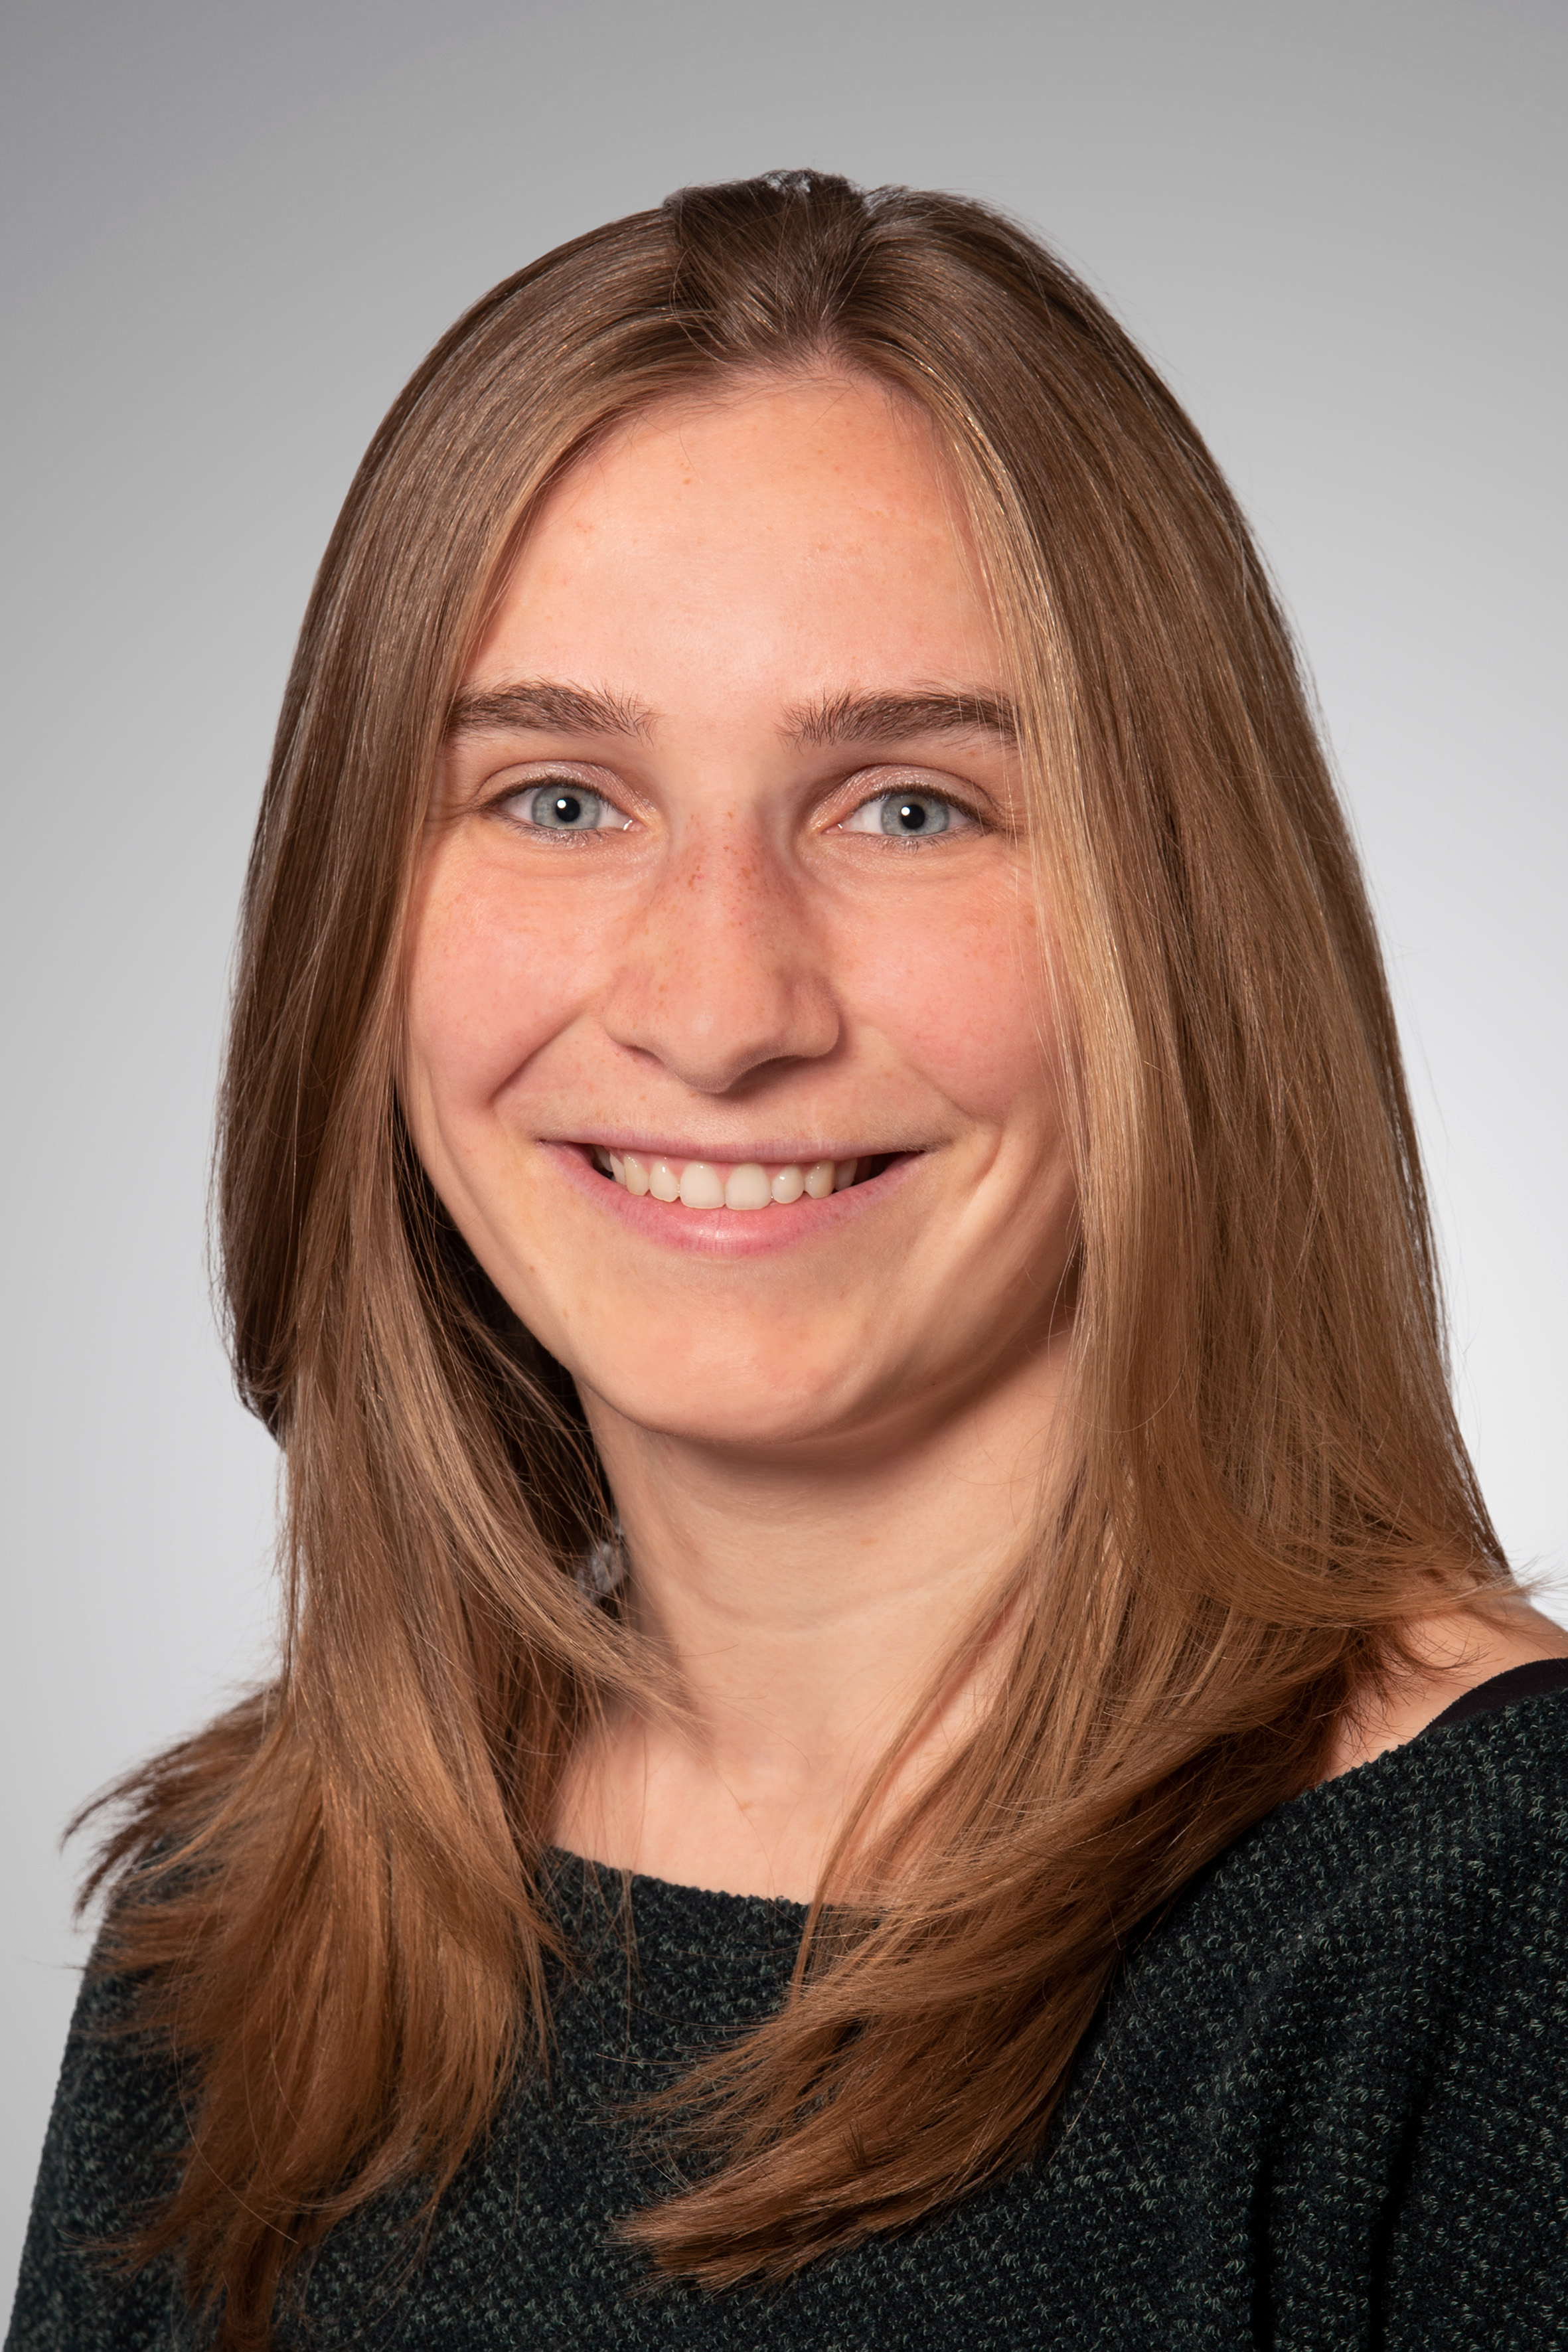
\includegraphics[width=\linewidth]{../resources/Profile_Picture.jpg}%	%trimming relative to image size

%---------------------------------------------------------------------------------------
%	META SKILLS
%----------------------------------------------------------------------------------------
  \fcolorbox{white}{white}{\begin{minipage}[c][1.5cm][c]{1\mpwidth}
    \LARGE{\textbf{\textcolor{darkcol}{Pauline Hasler}}} \\[2pt]
    \normalsize{ \textcolor{maincol} {Embedded Software Engineer} 
        \vspace{10pt}}
  \end{minipage}}

\renewcommand{\cvsection}[1]{
   \scalebox{0.95}[1]{\LARGE\bfseries \textcolor{darkcol}{#1}}

  \vspace{+5pt}
}



\cvsection{Kontakt}
\vspace{5pt}
\icontext{map-marker}{8mm}{Bungertenstrasse 12\\8307 Effretikon}{black}{lightaccentcol}\\[8pt]
\icontext{mobile}{8mm}{+41 78 695 64 19}{black}{lightaccentcol}\\[8pt]
\iconemail{envelope}{8mm}{pa.hasler@protonmail.com}{pa.hasler@protonmail.com}{black}{lightaccentcol}\\[8pt]
% \iconhref{github}{8mm}{github.com/hasler100}{https://github.com/Hasler100}{black}{lightaccentcol}\\[8pt]
\iconhref{linkedin}{8mm}{linkedin.com/pauline-hasler}{https://www.linkedin.com/in/pauline-hasler}{black}{lightaccentcol}\\

\vspace{+5pt}

\cvsection{{Programmiersprachen}}
    \cvskill{C} {Sehr gut} {0.8} \\[-2pt] % Für Firmware- und Applikationsentwicklung
    \cvskill{C++} {Erste Schritte} {0.2} \\[3pt] % Für Applikationen und Device-Treiber
    \cvskill{Python} {Grundlagen} {0.4} \\[-2pt]
\cvsection{Betriebssysteme}
    %\cvskill{Freertos} {Sehr gut} {0.8} \\[-2pt]
    \cvskill{Zephyr} {Gut} {0.6} \\[-2pt] % Schwerpunkt bytesatwork
    \cvskill{Yocto}{Erste Schritte} {0.2} \\[-2pt] % Schwerpunkt bytesatwork
    \cvskill{Linux/Windows (Desktop/Server)} {Grundwissen} {0.4} \\[-2pt] % Für embedded Linux
\cvsection{Tools}
    \cvskill{GitLab} {Gut} {0.6} \\[-2pt]
    %\cvskill{Jenkins} {Grundwissen} {0.4} \\[3pt]
    \cvskill{svn} {Gut} {0.6} \\[3pt]

\newpage
\cvsection{\\}
\cvsection{Sprachkenntnisse}
{  \vspace{-4pt}(Legasteniker)\\[6pt] }
    \cvskill{Deutsch} {Ausgezeichnet} {1} \\[-2pt] % Muttersprache, Voraussetzung bytesatwork
    \cvskill{Englisch} {Gut} {0.7} \\[3pt] % Für internationale Projekte
\cvsection{Soziale Kompetenzen}
    \icontext{caret-right}{4mm}{Teamplayer}{black}{accentcol}\\[6pt] % Teamorientierung bytesatwork
    \icontext{caret-right}{4mm}{Kommunikativ}{black}{accentcol}\\[6pt] % Kommunikation im Team
    \icontext{caret-right}{4mm}{Lösungsorientiert und hands-on}{black}{accentcol}\\[6pt] % Proaktive Arbeitsweise

\cvsection{Weitere Fähigkeiten}
    \icontext{caret-right}{4mm}{Visual Studio Code}{black}{accentcol}\\[6pt]
    \icontext{caret-right}{4mm}{Docker}{black}{accentcol}\\[6pt]
    %\icontext{caret-right}{4mm}{Polarion}{black}{accentcol}\\[6pt]
    %\icontext{caret-right}{4mm}{Führerschein Kategorie B1}{black}{accentcol}\\[6pt]
    \icontext{caret-right}{4mm}{CAD: Autodesk Inventor}{black}{accentcol}\\[6pt]

% hofixes to create fake-space to ensure the whole height is used

\renewcommand*\familydefault{\sfdefault}

\vspace{10pt}
\cvsection{Hobbys und Interessen}
    \icontext{caret-right}{4mm}{Bouldern}{black}{accentcol}\\[6pt]
    \icontext{caret-right}{4mm}{Kleinprojekte}{black}{accentcol}\\[6pt]
    \icontext{caret-right}{4mm}{Zeichnen}{black}{accentcol}\\[6pt]


%\cvqrcode{0.3}

\end{leftcolumn}
\begin{rightcolumn}

%---------------------------------------------------------------------------------------
%	PROFILE
%----------------------------------------------------------------------------------------
\cvsection{Biografie}

\cvtext{Ich habe Systemtechnik an der ZHAW mit Schwerpunkt Mechatronik studiert. Während des Studiums entdeckte ich meine Begeisterung für die Embedded-Software-Entwicklung. Seit Januar 2022 arbeite ich als Embedded Software Engineer bei der Baumer Group. Dort entwickelte ich mehrere Sensor-Firmwares in C und wirkte aktiv an der Weiterentwicklung des Frameworks mit. Besonders schätze ich die Möglichkeit, neue Technologien wie Zephyr-RTOS einzusetzen, sowie die enge Zusammenarbeit im Team.}

%---------------------------------------------------------------------------------------
%	EDUCATION
%----------------------------------------------------------------------------------------
\cvsection{Bildung}

\cvevent
    {09.2018 - 07.2021}
    {Bachelor of Science ZHF in Systemtechnik}
  {ZHAW Winterthur}
  {Vertiefung: Mechatronik \\ Bachelorarbeit: Multi-Level-TOF\\ Wahlfächer: Microcomputer Systems, Sensorik, Digitale Signalverarbeitung}

\cvevent
    {08.2017 - 07.2018}
    {Berufsmaturität 2}
    {Berufsfachschule Uster, ausrichtung: Technik}{}

%---------------------------------------------------------------------------------------
%	Berufserfahrung
%----------------------------------------------------------------------------------------

\cvsection{Berufserfahrung}

\cvevent
    {01.2022 -- heute}
    {Embedded Software Engineer}
  {Baumer Group: Firmware-Entwicklung für Sensoren}
  {Aufgabenbereiche: Entwicklung von Sensor-Firmware und Framework, insbesondere mit C und Zephyr-RTOS.Weiterentwicklung automatisierter Testverfahren sowie enge Zusammenarbeit im Team.}

\cvevent
    {07.2016 -- 08.2017}
    {Konstrukteur}
  {ELEX AG: Konstruktion / Konstruktive Projektleitung}
  {Aufgabenbereiche: Konstruktion von kundenspezifischen Elektrofiltern. Koordination von Teilprojekten mit Tochterfirmen.}

%---------------------------------------------------------------------------------------
%	Projekte und Praktika
%----------------------------------------------------------------------------------------

\cvsection{Projekte und Praktika}

\cvtext{Die Liste der Projekte und Praktika ist nicht vollständig. Weitere Tätigkeiten als Embedded Software Engineer sind im Zwischenzeugnis der Baumer Group aufgeführt. \\ }
  
\cvevent{}{OM60: Triangulationssensor}
    {Tools: Python, Anaconda, C, GitHub}
    {Der OM60 ist ein hochpräziser Triangulationssensor und der erste Sensor bei Baumer Frauenfeld, für den das neue Sensorframework eingesetzt wurde. Im Rahmen dieses Pilotprojekts, das mit agilen Methoden umgesetzt wurde, übernahm ich die Leitung der Firmware-Entwicklung. Ich war verantwortlich für die Sensorarchitektur, wobei eine robuste Firmware mit Echtzeitanforderungen und eine zuverlässige Datenkommunikation im Fokus standen.}

\cvevent{}{Application Template}
    {Tools: Python, Anaconda, C, GitHub\\Note: 5, 2er-Arbeit}
    {Basierend auf der OM60-Firmware wurde das Application Template entwickelt. Ziel war es, eine Basis für weitere Sensorprojekte zu schaffen, die die gängigen Schnittstellen und Funktionalitäten von Baumer-Sensoren abdeckt. Bei diesem Projekt arbeitete das gesamte Framework-Team gemeinsam an der optimalen Umsetzung. Besonders wichtig waren dabei die Modularität und die Codegrösse.}

\cvevent{}{Bachelorarbeit: Multi-Level-ToF}
    {Tools: Python, Anaconda, C, GitHub\\Note: 5, 2er-Arbeit}
    {In dieser Arbeit wurde die Auflösung einer Time-of-Flight-Kamera verbessert, indem Bilder mit unterschiedlichen Frequenzen aufgenommen und zu einem Bild kombiniert wurden. Zunächst wurden zwei Konzepte definiert, anschliessend der Messbereich der Kamera festgelegt und vermessen. Die gewonnenen Daten wurden mit einem Programm ausgewertet und die erwartete Verbesserung der Auflösung simuliert. Danach wurden die neuen Messverfahren implementiert, vermessen und mit den erwarteten Daten verglichen. Zudem wurde versucht, das neue Messverfahren zu optimieren und direkt in die Kamerafirmware zu integrieren.}
    \vfill\null

\cvevent{}{Projektarbeit: Flexibles Gelenk}
    {Tools: Python, ROS, GitHub\\Note: 5.5, 2er-Arbeit}
    {Es handelt sich um ein statisch unbestimmtes Gelenk, das durch Druckluft in verschiedene Positionen gesteuert werden kann. Bei gegebenem Kammerdruck und einer einwirkenden Kraft wurde der Winkel gemessen. Dies wurde für einen definierten Messbereich wiederholt. Anschliessend wurde anhand dieser Daten bei gegebenem Kammerdruck und Winkel die Kraft bestimmt. Abschliessend wurde ein Kraftfeedback implementiert, sodass bei einer bestimmten Krafteinwirkung (z. B. einem Schlag) eine Reaktion (z. B. Erschlaffen des Gelenks) ausgelöst wird.}

\cvevent{}{Praktikumsarbeiten: Mikrocontroller}
    {Tools: C, Keil uVision, Ubuntu, Yocto Project, SVN}
    {Praktika zu: Edge-Detektion, Power Management, Ansteuerung eines Bewegungssensors (DMA und Umgang mit Dateisystemen), Programmierung einer Eieruhr (Erstellung eines eigenen Schedulers, Umgang mit State-Maschinen, GPIO usw.)\hfill\break Auf Embedded Linux: Erste Schritte mit Yocto, Erstellen eines Kernel-Moduls, Handschrifterkennung, Embedded Machine Learning, Scheduling, Ansteuerung von GPIOs.}
  
\cvevent{}{Praktikumsarbeiten: Computertechnik}
    {Tools: Assembly, C, Keil uVision}
    {Ansteuerung von Schaltern und Lampen mit Memory-Maps, Addieren und Multiplizieren unter Berücksichtigung von Flags, Umgang mit Interrupts, Sichern und Wiederherstellen von Registerwerten in Unterprogrammen, Umgang mit Timern, ADC, GPIO, UART und SPI, Erstellen von endlichen Zustandsautomaten (Finite State Machines).}
  
\cvevent{}{Praktikumsarbeiten: Weiteres}
    {Tools: C++, Matlab, Simulink, Mbed, Assembly, GitHub, SVN usw. }
    {Der Systemtechnikunterricht ist äusserst vielfältig, da Informatik, Mechanik und Elektronik unterrichtet werden. Besonders an der ZHAW ist der praktikumsbegleitende Unterricht, durch den ich viele weitere praktische Erfahrungen sammeln konnte. Dazu gehören unter anderem: \\
    Balancieren eines Würfels auf einer Kante durch Schwungrad, Regelung einer Kugelwippe, eines Wasserstandes oder weiterer Systeme (Regelungstechnik), \\
    Erstellen von Spektrogrammen, Filterung von digitalen und analogen Signalen, Hinzufügen und Filtern von Schall auf Tonaufnahmen (Digitale Signalverarbeitung), \\
    Ausmessung und Verhaltensanalysen verschiedenster Sensoren (Sensortechnik), \\
    Programmierung von Industrie- und mobilen Robotern, Erstellen von Karten durch Gyrosensor (Robotik).}


%---------------------------------------------------------------------------------------
%	Publikationen
%----------------------------------------------------------------------------------------
%\cvsection{Publikationen}

%---------------------------------------------------------------------------------------
%	Referenzen
%----------------------------------------------------------------------------------------
\cvsection{Referenzen}

\cvtext{Referenzen sind auf Anfrage erhältlich.\\ }


\vspace{1cm}

Effretikon, den \today     \hspace{1cm}   \hrulefill


\hspace*{30mm}\phantom{Effretikon, den \today }

\end{rightcolumn}
\end{paracol}

\end{document}
